\section{Introduction}\label{sec:Intro}

\subsection*{Bits dropped in form elsewhere}

The developments of a Unifying Theory of Programming (UTP)
can involve a number of false starts,
as alphabet variables are chosen
and semantics and healthiness conditions are defined.
Typically, some calculations done just to check that everything
is fine in fact reveal problems with the theory.
So we iterate by revising the basic definitions,
and attempting the calculations again.
Hopefully, these eventually converge to what becomes a sound and useful
UTP Theory.
In a recent bout of such theory revision and re-calculation,
which required five iterations in total,
the author noted that common patterns of proof-steps kept occurring
in each iteration.

The way the calculator is designed to be used is
that a function implementing a calculator Read-Execute-Print-Loop (REPL)
is given a dictionary and starting predicate as inputs.
It then offers the user the opportunity to invoke various
commands to perform calculation steps.
The user can then indicate when they are finished,
at which point the calculator function returns
a data-structure that logs the complete calculation outcome.


The first property of interest for this calculator
was calculating the effect of $run(A \pseq B)$,
where $A$ and $B$ were atomic action predicates with alphabet $\setof{s,s'}$.
For convenience we predefined the predicate $A \pseq B$, as
\begin{code}
athenb = pseq [patm (pvar "A"),patm (pvar "B")]
\end{code}
We then invoke the calculator as follows,
\begin{code}
calcREPL dictUTCP (run athenb)
\end{code}
and proceed to interact
(here the prompt  ``\texttt{ ?,d,r,l,s,c,u,x :-}''
shows the available commands)
\begin{verbatim}
UTCP-0.7, UTP-Calc v0.0.1
run(A(A) ;; A(B))
 ?,d,r,l,s,c,u,x :- d
 = "defn. of run.3"
   (A(A) ;; A(B))[g::,lg,lg,lg:/g,in,ls,out]
 ; ~ls(lg:) * (A(A) ;; A(B))[g::,lg,lg:/g,in,out]
 ?,d,r,l,s,c,u,x :- d
 = "defn. of ;;"
   (A(A)[g:1,lg/g,out] \/
   A(B)[g:2,lg/g,in])[g::,lg,lg,lg:/g,in,ls,out]
 ; ~ls(lg:) * (A(A) ;; A(B))[g::,lg,lg:/g,in,out]
 ?,d,r,l,s,c,u,x :- s
 = "simplify"
   A(A)[g:::1,lg,lg,lg::/g,in,ls,out] \/
   A(B)[g:::2,lg::,lg,lg:/g,in,ls,out]
 ; ~ls(lg:) * (A(A) ;; A(B))[g::,lg,lg:/g,in,out]
.... 10 more steps
 ?,d,r,l,s,c,u,x :- r
 = "ls'-cleanup"
(A ; B) /\ ls' = {lg:}
\end{verbatim}
The user simply indicates the broad class of command required,
and the calculator works on the current goal predicate.
A text transcript is produced,
which is essentially the above
without the prompts.
The marking facility, requiring the \texttt{Pred}/\texttt{MPred} complication,
is currently used when displaying the transcript in a terminal
window to highlight old and new parts of predicates as changes are made.
Currently this only works well on the Mac OS X terminal,
because it seems to be the only one that properly supports ANSI escape sequences.

\subsection{Research Context}\label{ssec:context}

We have recently started to explore using UTP
to do the  formal modelling of a language,
called ``Process Modelling Language'' (PML),
designed to describe software development and similar business
processes \cite{DBLP:journals/infsof/AtkinsonWN07}.
The main objective is to give PML a formal semantics,
as the basis for a number of analysis tools that could be made available
to process designers and users---with one key application
area being the modelling of clinical healthcare pathways.
It quickly became apparent that PML and similar (business) process
notations essentially involve concurrency with global shared mutable state.

There has been work using UTP
to model concurrent programs with shared mutable state,
most notably
with an encoding into action systems having been done by
Woodcock and Hughes\cite{DBLP:conf/icfem/WoodcockH02}.
We have been looking at adapting this work to provide a UTP semantics
for PML.
%In addition, we have started to take an interest in the ``Views'' paper
%by Dinsdale-Young and colleagues\cite{conf/popl/Dinsdale-YoungBGPY13},
%that provides a framework within which it is possible
%to construct instances of many different concurrency theories,
%ranging from
%type-theory \cite{tal-toplas,Smit00b,journals/fuin/AhmedFM07},
%Owicki-Gries\cite{Owicki76},
%separation logic\cite{conf/lics/CalcagnoOY07}
%and rely-guarantee\cite{Jones83}
%approaches,
%among others.

So we started by taking the action-system UTP semantics for Unifying Theories
of Parallel Programming (UTPP) \cite{DBLP:conf/icfem/WoodcockH02},
and reworking it to use a system for generating unique labels,
in order to give a slight improvement to the compositionality
of the semantics. This we call a Unifying Theory of Concurrent Programming
(UTCP) and details of this are,
at the time of writing,
accepted for publication\cite{conf/tase/BMN16}.
We give a very brief overview here of this theory.
The language assumes atomic actions ($A$) that modify a generic state,
and four composition operators: sequential ($\lseq$), parallel ($\parallel$),
non-deterministic choice ($\pcond$) and non-deterministic iterations ($\piter{}$)
\[
   P ::= A \mid P \pseq P \mid P \parallel P \mid P \pcond P \mid \piter P
\]
Note that this is essentially the same as the baseline ``Command'' language
in the Views paper\cite{conf/popl/Dinsdale-YoungBGPY13}.
In UTCP we have two distinct groups of observations:
\begin{itemize}
  \item
    Variables that track changes during execution
    (dynamic observations),
    modelling the generic state ($s,s'$)
    and the global label-set ($ls,ls'$) used to manage control-flow.
  \item
    Variables that record static parameters such as start ($in$)
    and stop ($out$) labels for a construct,
    as well as a label generator ($g$) associated with each construct.
\end{itemize}
So our UTCP theory is based on a non-homogeneous relation
with alphabet $s$, $s'$, $ls$, $ls'$, $g$, $in$, and $out$.


\subsection{Theory Construction Difficulties}\label{ssec:difficulties}

The theory with its somewhat unusual arrangement of observation variables
did \emph{not} emerge as an immediate and obvious solution.
The theory design started with an homogeneous alphabet with $g'$, $in'$ and $out'$
being present.
Semantic definitions were proposed for all constructs,
and then a series of calculations were undertaken in order to check
the validity of those definitions.
The first such calculation was that of the semantics of a single atomic
action ($A$), and this always seemed to work out fine.
The second calculation was of the sequential composition of two atomic
actions ($A\pseq B$), and this is where problems arose.

The first problem was relatively minor
---a lot of the semantics talks about the presence of various
labels in the global label-set, or alternatively, their  absence,
and of modifications to that set.
This resulted in very wide expressions,
so some shorthand notations were introduced:
using $\ell$ to denote singleton set $\setof\ell$;
or writing $ls(L)$ instead of $L \subseteq ls$, for example.

The second problem was more serious.
The calculation to take $A \pseq B$,
expand it using the semantics of $\pseq$,
and reduce it down to a simple predicate that described the fairly obvious
correct behaviour,
was very lengthy.
Often it would give the right result,
but then checking $A \parallel B$ (an even longer calculation)
would give an incorrect answer.
In every case the fault was traced back to sequential composition%
\footnote{
In the author's experience,
when building semantic theories involving concurrency or parallelism,
it is always sequential composition that causes the most difficulty
}
,
where either the definition of $\pseq$ was wrong,
or, as proved crucial,
the behaviour of ``standard'' UTP sequential composition
was at fault.
The calculations for sequential and parallel composition
required typically about 400 lines of \LaTeX\ and resulted
in 7 full pages of output,
an extract of which is shown in Fig. \ref{fig:attempt4}.

\begin{figure}
  \centering
  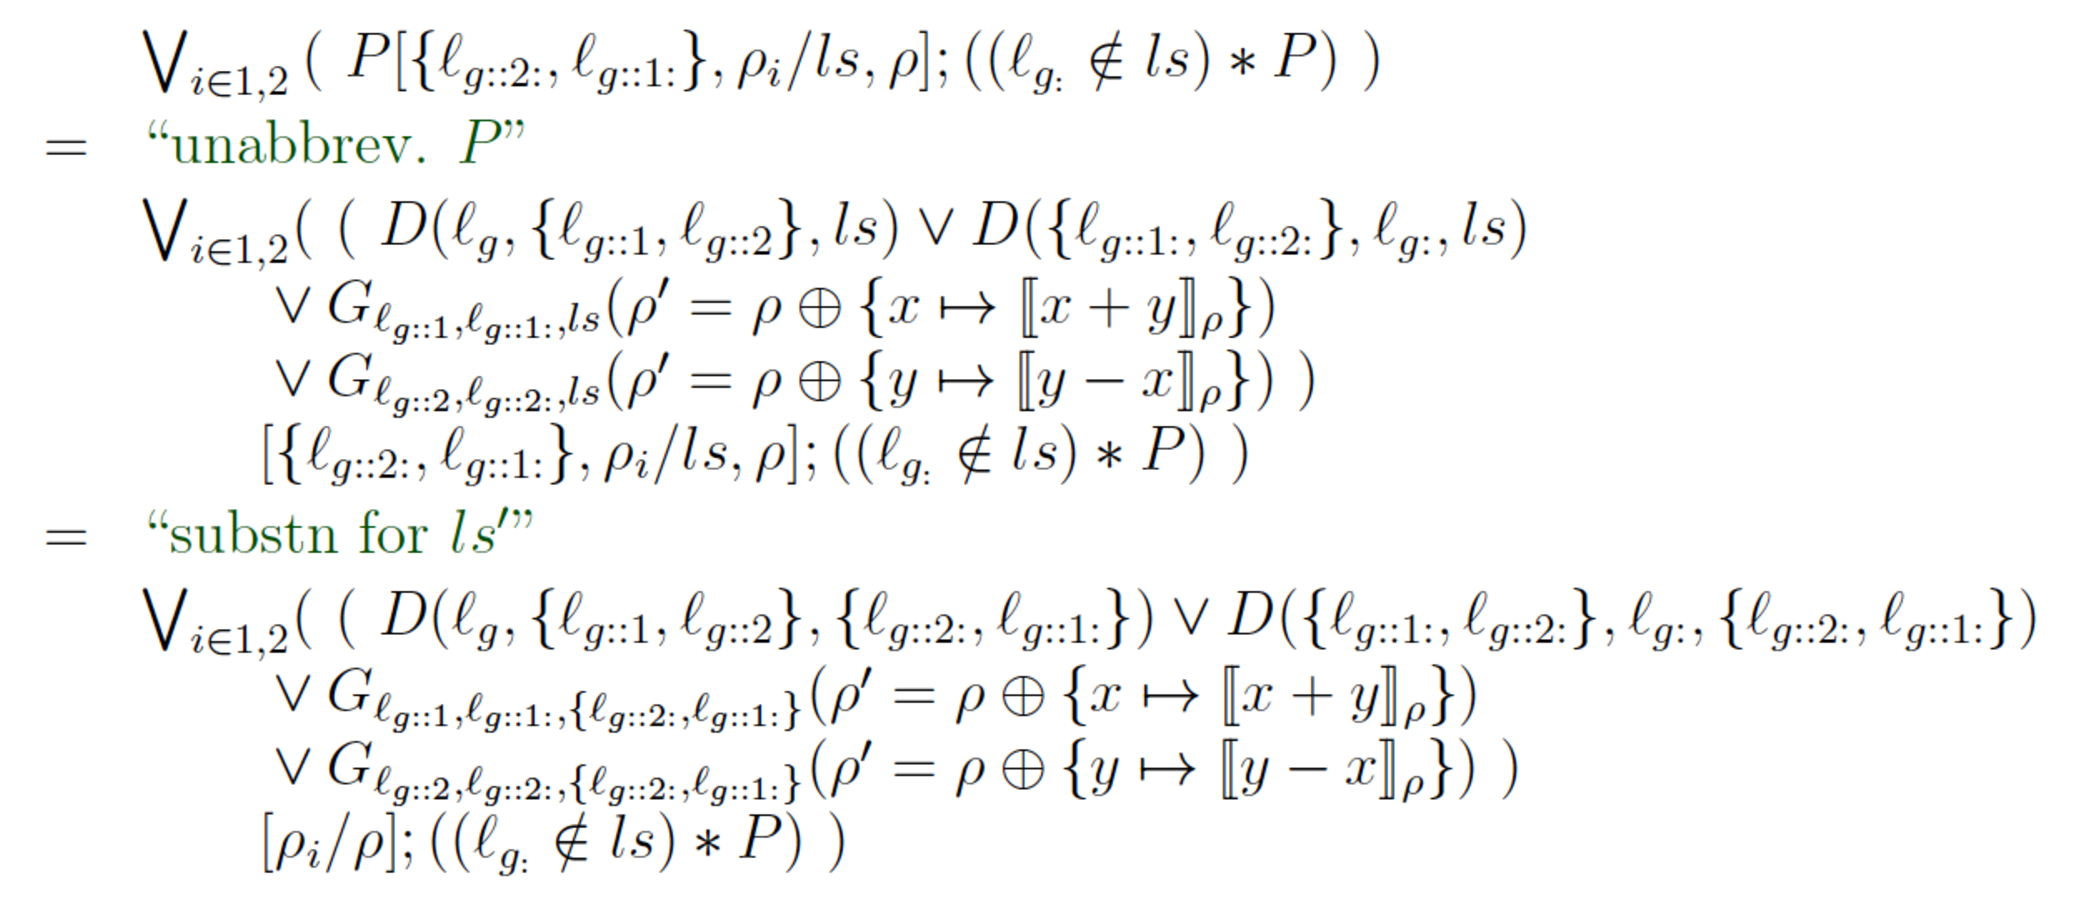
\includegraphics[width=4.5in]{Attempt4.eps}\\
  \caption{Extract from 4th attempt to calculate $x:=x+y \parallel y:=y-x$}
  \label{fig:attempt4}
\end{figure}

With choice and iteration to be covered,
it was becoming very clear that a better way was required
for checking semantic outcomes.

\subsection{A Plan}\label{ssec:plan}

We briefly considered using the \UTP2 theorem prover
\cite{DBLP:conf/utp/Butterfield10,DBLP:conf/utp/Butterfield12},
but it would have required a lot of setup effort,
and it is currently not in an ideal state%
\footnote{The issue has to do with difficulties installing
the relevant software libraries
on more recent versions of Haskell.}
.
However, as part of our work on the formal semantics of PML,
we had developed a parser and some initial analysis tools
in Haskell\cite{Haskell2010},
and this software contained abstract syntax and support
for general predicates.
It became really obvious that this could be quickly adapted,
to mechanise the checking calculations, that were being performed
during each attempt.
In particular,
the key inspiration was the observation,
over all of those calculation attempts (five in all!),
that the pattern of each calculation was very uniform and similar.
So a decision was taken to construct the calculator described in this paper.



\subsection{Structure of this paper}

In Sect. \ref{sec:Design}
we describe key design decisions
that underlie the calculator's features,
and which are responsible for its success.
Then, in Sect. \ref{sec:Theorising}
we present a development of a theory using the calculator,
as a way of describing its features, from a user's perspective.
This is followed by a short example of the calculator in use
(Sect. \ref{sec:Using}).
We then discuss this calculator, and related work
and draw some conclusions in Sect. \ref{sec:Conc},
before finishing up describing future plans for the calculator.
